% Options for packages loaded elsewhere
\PassOptionsToPackage{unicode}{hyperref}
\PassOptionsToPackage{hyphens}{url}
\PassOptionsToPackage{dvipsnames,svgnames,x11names}{xcolor}
%
\documentclass[
  letterpaper,
  DIV=11,
  numbers=noendperiod]{scrreprt}

\usepackage{amsmath,amssymb}
\usepackage{iftex}
\ifPDFTeX
  \usepackage[T1]{fontenc}
  \usepackage[utf8]{inputenc}
  \usepackage{textcomp} % provide euro and other symbols
\else % if luatex or xetex
  \usepackage{unicode-math}
  \defaultfontfeatures{Scale=MatchLowercase}
  \defaultfontfeatures[\rmfamily]{Ligatures=TeX,Scale=1}
\fi
\usepackage{lmodern}
\ifPDFTeX\else  
    % xetex/luatex font selection
\fi
% Use upquote if available, for straight quotes in verbatim environments
\IfFileExists{upquote.sty}{\usepackage{upquote}}{}
\IfFileExists{microtype.sty}{% use microtype if available
  \usepackage[]{microtype}
  \UseMicrotypeSet[protrusion]{basicmath} % disable protrusion for tt fonts
}{}
\makeatletter
\@ifundefined{KOMAClassName}{% if non-KOMA class
  \IfFileExists{parskip.sty}{%
    \usepackage{parskip}
  }{% else
    \setlength{\parindent}{0pt}
    \setlength{\parskip}{6pt plus 2pt minus 1pt}}
}{% if KOMA class
  \KOMAoptions{parskip=half}}
\makeatother
\usepackage{xcolor}
\usepackage[top=3cm,left=3cm,right=2cm,bottom=2cm]{geometry}
\setlength{\emergencystretch}{3em} % prevent overfull lines
\setcounter{secnumdepth}{5}
% Make \paragraph and \subparagraph free-standing
\ifx\paragraph\undefined\else
  \let\oldparagraph\paragraph
  \renewcommand{\paragraph}[1]{\oldparagraph{#1}\mbox{}}
\fi
\ifx\subparagraph\undefined\else
  \let\oldsubparagraph\subparagraph
  \renewcommand{\subparagraph}[1]{\oldsubparagraph{#1}\mbox{}}
\fi


\providecommand{\tightlist}{%
  \setlength{\itemsep}{0pt}\setlength{\parskip}{0pt}}\usepackage{longtable,booktabs,array}
\usepackage{calc} % for calculating minipage widths
% Correct order of tables after \paragraph or \subparagraph
\usepackage{etoolbox}
\makeatletter
\patchcmd\longtable{\par}{\if@noskipsec\mbox{}\fi\par}{}{}
\makeatother
% Allow footnotes in longtable head/foot
\IfFileExists{footnotehyper.sty}{\usepackage{footnotehyper}}{\usepackage{footnote}}
\makesavenoteenv{longtable}
\usepackage{graphicx}
\makeatletter
\def\maxwidth{\ifdim\Gin@nat@width>\linewidth\linewidth\else\Gin@nat@width\fi}
\def\maxheight{\ifdim\Gin@nat@height>\textheight\textheight\else\Gin@nat@height\fi}
\makeatother
% Scale images if necessary, so that they will not overflow the page
% margins by default, and it is still possible to overwrite the defaults
% using explicit options in \includegraphics[width, height, ...]{}
\setkeys{Gin}{width=\maxwidth,height=\maxheight,keepaspectratio}
% Set default figure placement to htbp
\makeatletter
\def\fps@figure{htbp}
\makeatother

\usepackage{booktabs}
\usepackage{longtable}
\usepackage{array}
\usepackage{multirow}
\usepackage{wrapfig}
\usepackage{float}
\usepackage{colortbl}
\usepackage{pdflscape}
\usepackage{tabu}
\usepackage{threeparttable}
\usepackage{threeparttablex}
\usepackage[normalem]{ulem}
\usepackage{makecell}
\usepackage{xcolor}
\KOMAoption{captions}{tableheading,figureheading}
\makeatletter
\@ifpackageloaded{caption}{}{\usepackage{caption}}
\AtBeginDocument{%
\ifdefined\contentsname
  \renewcommand*\contentsname{Índice}
\else
  \newcommand\contentsname{Índice}
\fi
\ifdefined\listfigurename
  \renewcommand*\listfigurename{Lista de Figuras}
\else
  \newcommand\listfigurename{Lista de Figuras}
\fi
\ifdefined\listtablename
  \renewcommand*\listtablename{Lista de Tabelas}
\else
  \newcommand\listtablename{Lista de Tabelas}
\fi
\ifdefined\figurename
  \renewcommand*\figurename{Figura}
\else
  \newcommand\figurename{Figura}
\fi
\ifdefined\tablename
  \renewcommand*\tablename{Tabela}
\else
  \newcommand\tablename{Tabela}
\fi
}
\@ifpackageloaded{float}{}{\usepackage{float}}
\floatstyle{ruled}
\@ifundefined{c@chapter}{\newfloat{codelisting}{h}{lop}}{\newfloat{codelisting}{h}{lop}[chapter]}
\floatname{codelisting}{Listagem}
\newcommand*\listoflistings{\listof{codelisting}{Lista de Listagens}}
\makeatother
\makeatletter
\makeatother
\makeatletter
\@ifpackageloaded{caption}{}{\usepackage{caption}}
\@ifpackageloaded{subcaption}{}{\usepackage{subcaption}}
\makeatother
\ifLuaTeX
\usepackage[bidi=basic]{babel}
\else
\usepackage[bidi=default]{babel}
\fi
\babelprovide[main,import]{portuguese}
% get rid of language-specific shorthands (see #6817):
\let\LanguageShortHands\languageshorthands
\def\languageshorthands#1{}
\ifLuaTeX
  \usepackage{selnolig}  % disable illegal ligatures
\fi
\usepackage{bookmark}

\IfFileExists{xurl.sty}{\usepackage{xurl}}{} % add URL line breaks if available
\urlstyle{same} % disable monospaced font for URLs
\hypersetup{
  pdftitle={Trabalho MLG},
  pdfauthor={Eliana Cardoso Gonçalves e Sophia Araujo de Moraes},
  pdflang={pt},
  colorlinks=true,
  linkcolor={blue},
  filecolor={Maroon},
  citecolor={Blue},
  urlcolor={Blue},
  pdfcreator={LaTeX via pandoc}}

\title{Trabalho MLG}
\author{Eliana Cardoso Gonçalves e Sophia Araujo de Moraes}
\date{26/08/2024}

\begin{document}
\maketitle

\renewcommand*\contentsname{Índice}
{
\hypersetup{linkcolor=}
\setcounter{tocdepth}{2}
\tableofcontents
}
\chapter{Dados da Penn World Table de
2020}\label{dados-da-penn-world-table-de-2020}

Dois tópicos desse estudo (MODELO LINEAR NORMAL e MODELO GAMA
LOG-LINEAR) se concentram em uma amostra de 183 países distintos no ano
de 2014. Os dois modelos foram utilizados para explorar como a força de
trabalho e o estoque de capital influenciam o PIB, desse modo por meio
de regressões lineares múltiplas, será estimado os coeficientes que
quantificam essas relações, permitindo-nos compreender melhor os
determinantes do crescimento econômico.

Essa relação pode ser expressa pela seguinte equação:

\[Y=β0+β1X1+β2X2+...+βpXp+ε\]

Onde:

\begin{itemize}
\item
  \(Y\) é a variável dependente ( PIB Nacional (Y) em dólares PPP de
  2014).
\item
  \(X1,X2,...,Xp\) são as variáveis independentes ( Força de Trabalho
  (L)e o Estoque de Capital (K) em dólares PPP de 2014).
\item
  \(β1,β2,...,βp\) são os coeficientes de regressão que representam os
  efeitos das variáveis independentes na variável dependente.
\item
  \(ε\) é o termo de erro, que representa a variação não explicada pelo
  modelo.
\end{itemize}

Para complementar a análise, é importante entender como os dois modelos
--- o Modelo Linear Normal e o Modelo Gama Log-Linear --- foram
utilizados para explorar as relações entre o PIB nacional, a força de
trabalho e o estoque de capital. Esses modelos oferecem diferentes
abordagens para analisar os dados e podem fornecer insights valiosos
sobre os fatores que impulsionam o crescimento econômico:

\textbf{Modelo Linear Normal}: O Modelo Linear Normal é uma aplicação
clássica da regressão linear múltipla. Neste contexto, assume-se que a
relação entre as variáveis independentes (força de trabalho e estoque de
capital) e a variável dependente (PIB) é linear. Isso significa que cada
incremento em uma variável independente resulta em um aumento ou
diminuição constante na variável dependente, dependendo do sinal e do
valor dos coeficientes de regressão.

Este modelo é baseado em algumas suposições, como a normalidade dos
resíduos, homocedasticidade (ou seja, a variância constante dos
resíduos), e a ausência de multicolinearidade entre as variáveis
independentes. Quando essas suposições são satisfeitas, o Modelo Linear
Normal fornece estimativas consistentes e eficientes dos coeficientes de
regressão, permitindo uma compreensão clara de como cada fator contribui
para o PIB.

\textbf{Modelo Gama Log-Linear}: Por outro lado, o Modelo Gama
Log-Linear oferece uma abordagem alternativa, especialmente útil quando
os dados não atendem às suposições de normalidade e homocedasticidade do
modelo linear. Este modelo é particularmente apropriado para situações
onde a variável dependente (PIB) assume valores positivos e pode
apresentar uma distribuição assimétrica, o que é comum em dados
econômicos.

No Modelo Gama Log-Linear, a transformação logarítmica é aplicada à
variável dependente. Isso permite capturar relações não lineares entre o
PIB e as variáveis independentes, como a força de trabalho e o estoque
de capital. A distribuição Gama, utilizada nesse modelo, é adequada para
modelar a variável dependente em casos onde há heterocedasticidade ---
ou seja, quando a variabilidade dos dados aumenta com o valor previsto.

Essa abordagem é especialmente útil para capturar efeitos
multiplicativos, onde as variáveis independentes influenciam a variável
dependente de forma proporcional, em vez de aditiva. O Modelo Gama
Log-Linear pode, portanto, revelar nuances e complexidades na relação
entre os fatores estudados e o crescimento econômico que o modelo linear
normal pode não captar.

\section{Modelo Linear Normal}\label{modelo-linear-normal}

\begin{longtable}[t]{l>{\raggedleft\arraybackslash}p{17em}rr}

\caption{\label{tbl-t1}Tabela Resumo das Variáveis Y, L e K.}

\tabularnewline

\toprule
 & K & L & Y\\
\midrule
Mean & 3058761.263 & 54.6094443 & 769941.411\\
Std.Dev & 8413105.576 & 196.3877082 & 2264112.549\\
Min & 7345.099 & 0.2993725 & 2569.155\\
Median & 394840.953 & 11.6562212 & 123419.395\\
Max & 64118472.000 & 2045.9122435 & 18244220.000\\
\bottomrule

\end{longtable}

\begin{figure}

\caption{\label{fig-y}Histograma PIB Nacional (Y) em dólares PPP de
2014}

\centering{

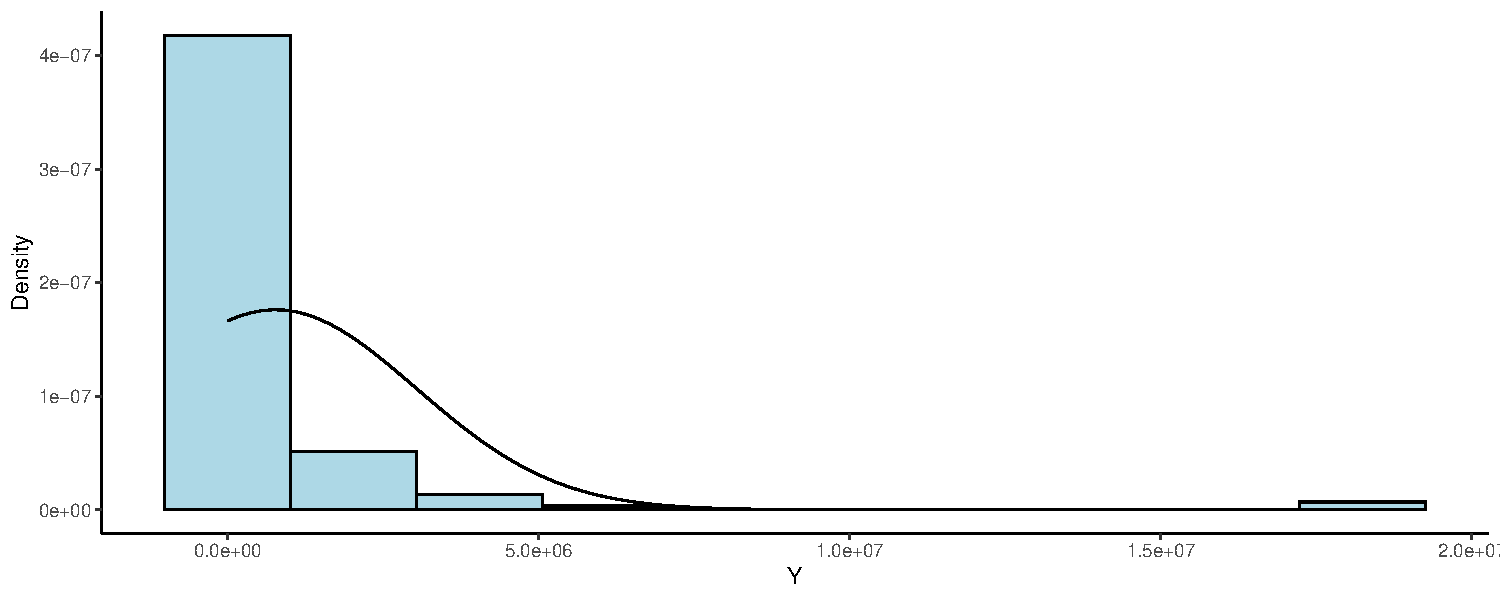
\includegraphics{trabalho_files/figure-pdf/fig-y-1.pdf}

}

\end{figure}%

Observando o Figura~\ref{fig-y} e Tabela~\ref{tbl-t1} , o valor mínimo
do PIB é \$2.569, enquanto o valor máximo é significativamente maior,
chegando a \$18.244.220, indicando uma grande variação no PIB entre os
países da amostra.A média do PIB é \$769.941, o que é substancialmente
maior que a mediana de \$123.419, sugerindo que alguns países com PIB
muito alto estão puxando a média para cima. A distribuição do PIB é
bastante assimétrica, com muitos países tendo PIBs relativamente baixos
e poucos países com PIBs muito altos.

\begin{figure}

\caption{\label{fig-l}Histograma Força de Trabalho (L)}

\centering{

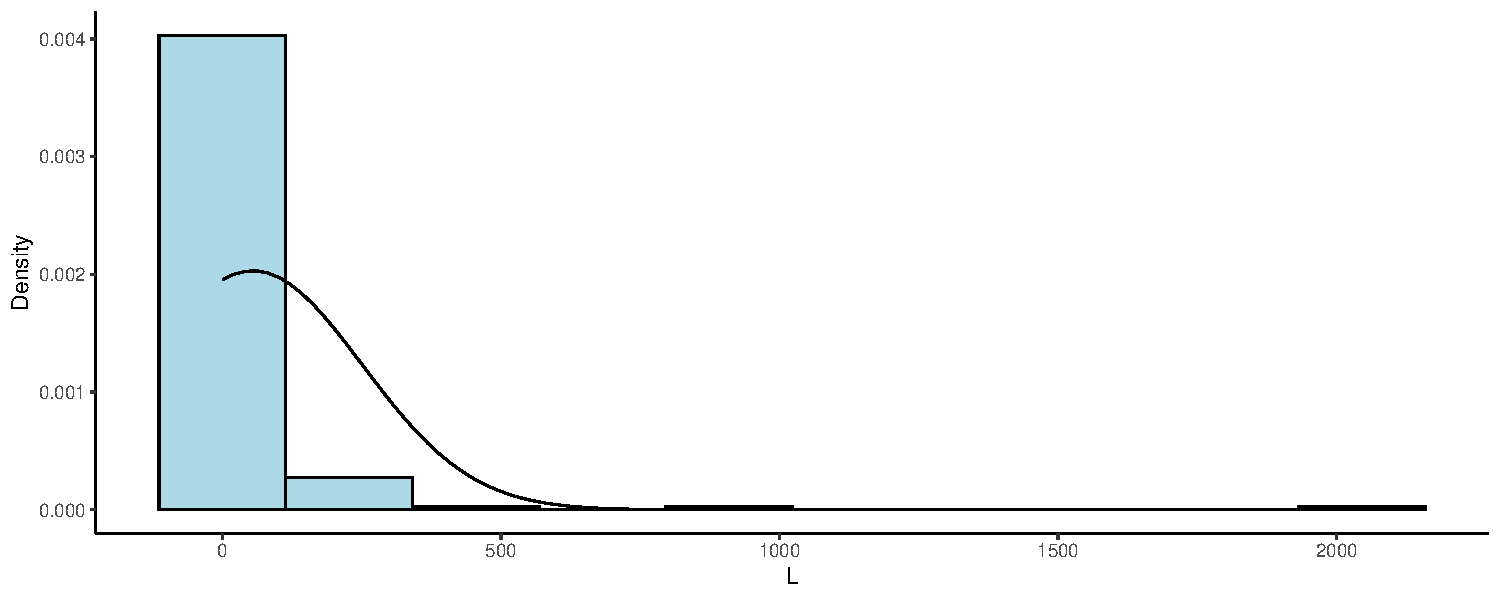
\includegraphics{trabalho_files/figure-pdf/fig-l-1.pdf}

}

\end{figure}%

Analisando o Figura~\ref{fig-l} e a Tabela~\ref{tbl-t1}, a variação da
força de trabalho de 0,2994 a 2.045,91 reflete uma grande disparidade na
população economicamente ativa entre os países. Com uma média de 54,60 e
uma mediana de 11,65, a distribuição mostra-se assimétrica, sugerindo a
presença de países com forças de trabalho extremas, seja pela sua
grandeza ou pequenez em relação à média da amostrm alguns países com
países com a força de trabalho outlier.

\begin{figure}

\caption{\label{fig-k}Histograma Estoque de Capital (K) em dólares PPP
de 2014)}

\centering{

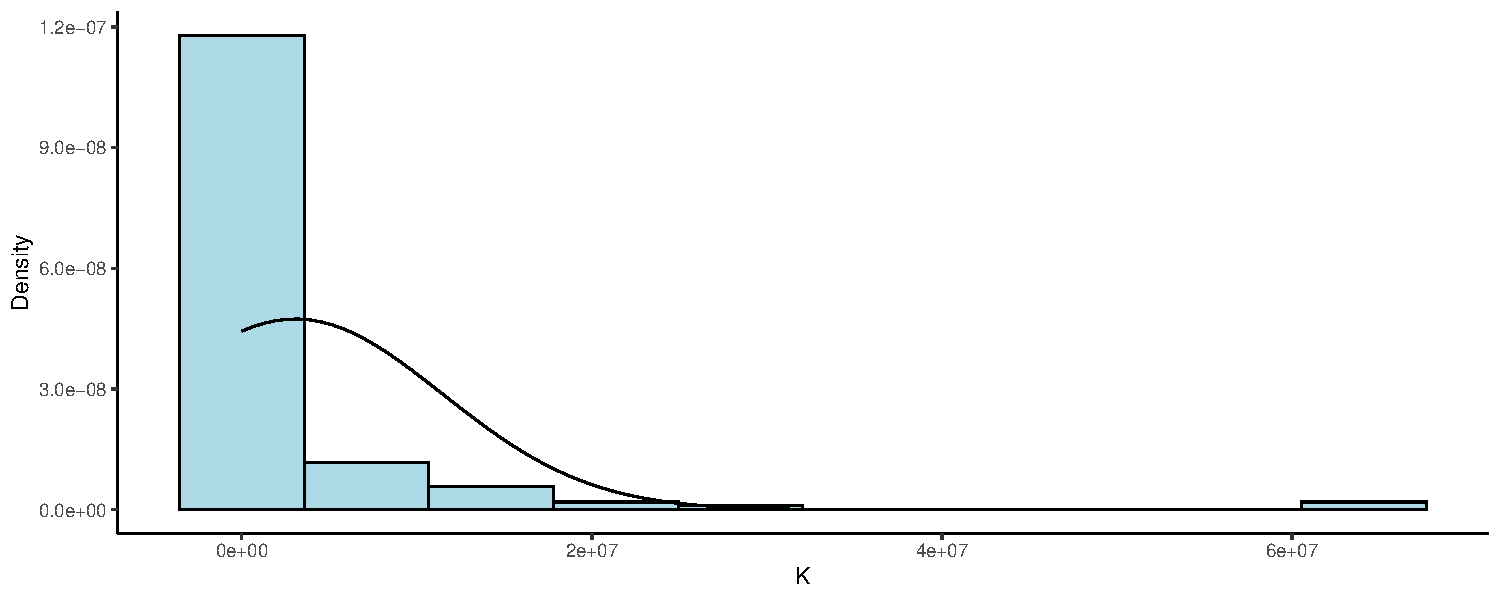
\includegraphics{trabalho_files/figure-pdf/fig-k-1.pdf}

}

\end{figure}%

Analisando os valores da Tabela~\ref{tbl-t1} e Figura~\ref{fig-k} ,
observamos que o estoque de capital varia amplamente, de \$7.345 a
\$64.118.472, indicando diferenças significativas no nível de
investimento em capital produtivo entre os países.

A média do estoque de capital é \$3.058.761, consideravelmente maior que
a mediana de \$394.841, o que sugere que alguns países têm estoques de
capital extremamente altos que estão elevando a média.

\subsection{Resultados}\label{resultados}

Para garantir a robustez e confiabilidade dos resultados, optamos por
realizar uma transformação log-log nas variáveis, considerando que o PIB
Nacional (Y) em dólares PPP de 2014, juntamente com as variáveis
independentes ``força de trabalho'' e ``estoque de capital'', não
apresentam uma distribuição normal. Essa abordagem vai permitir que aos
pressupostos do modelo normal sejam atendidos e obter resultados mais
consistentes.

Ao aplicar a transformação log-log, estamos ajustando a distribuição das
variáveis para se adequarem melhor ao modelo, mitigando quaisquer
distorções ou viés que possam surgir devido à falta de normalidade. Isso
nos permite realizar inferências estatísticas mais confiáveis e
interpretar os efeitos das variáveis independentes sobre o PIB Nacional
de forma mais precisa.

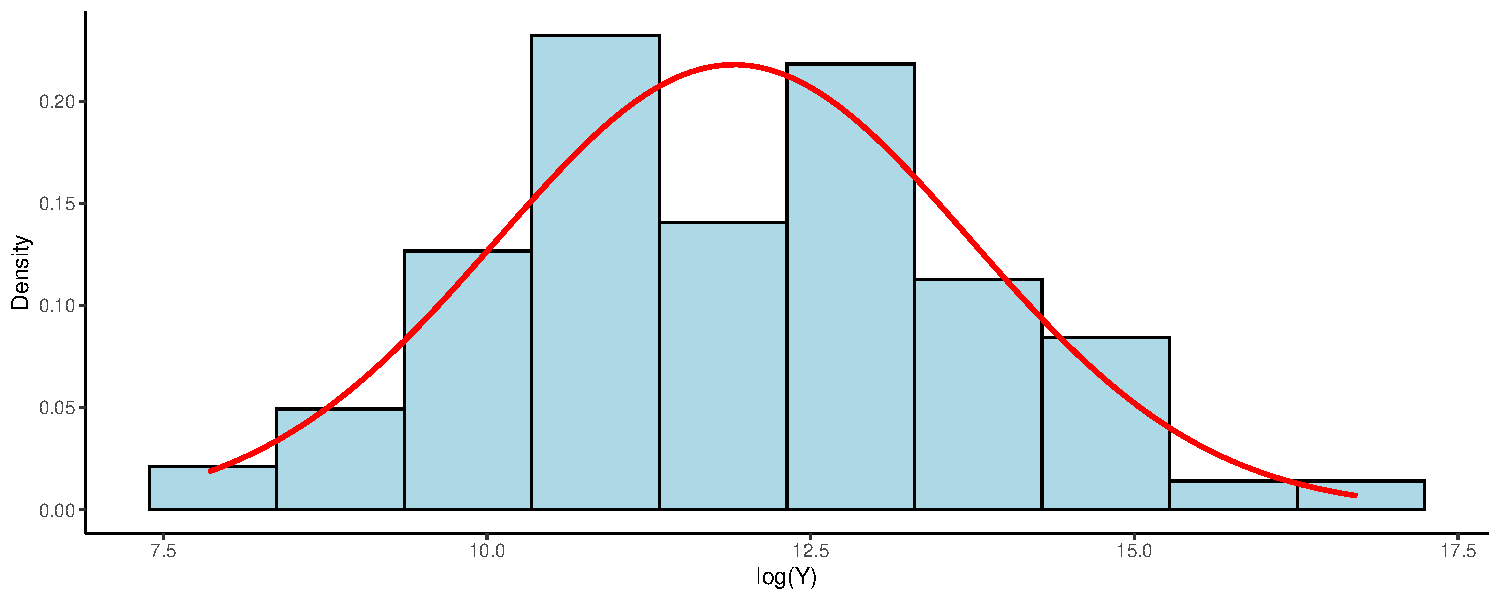
\includegraphics{trabalho_files/figure-pdf/unnamed-chunk-9-1.pdf}

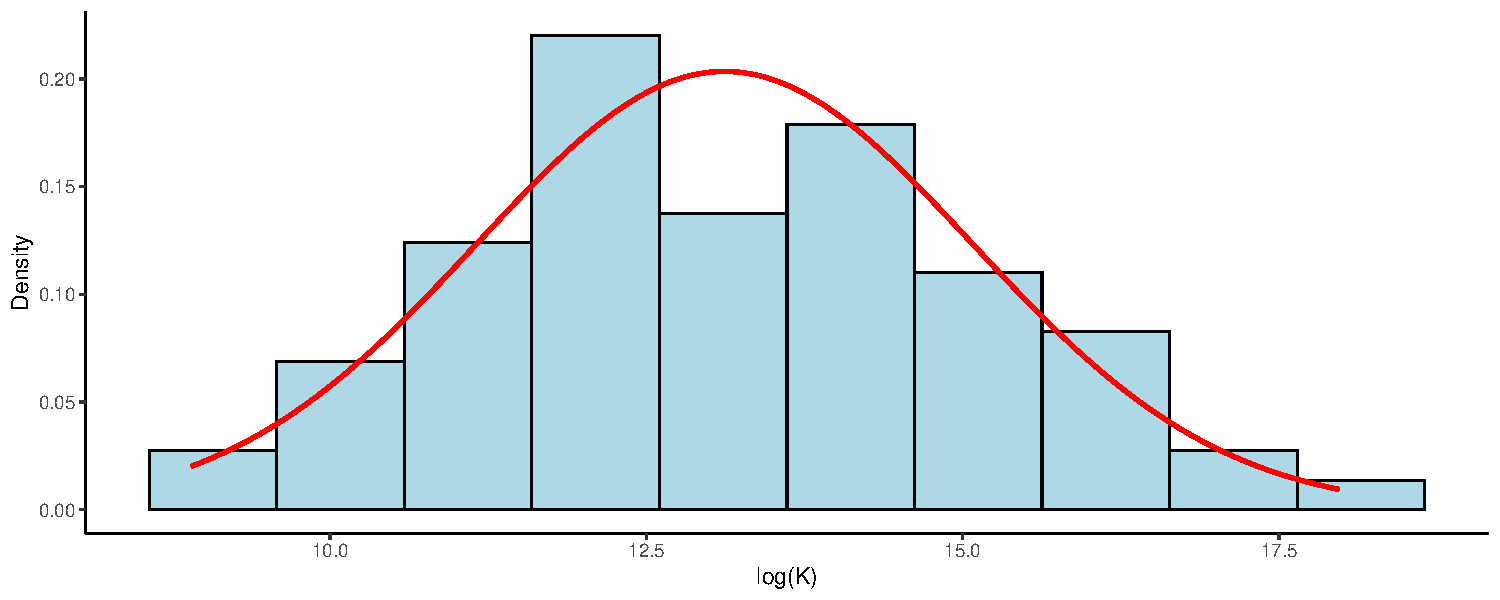
\includegraphics{trabalho_files/figure-pdf/unnamed-chunk-10-1.pdf}

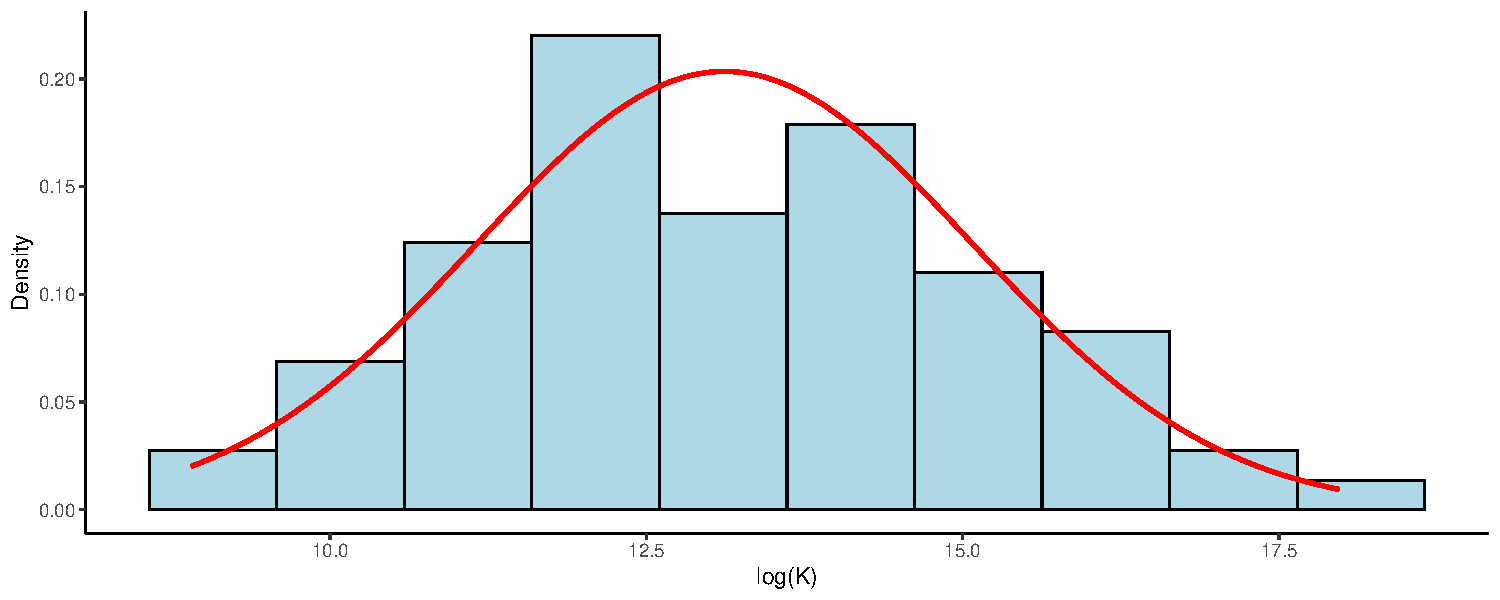
\includegraphics{trabalho_files/figure-pdf/unnamed-chunk-11-1.pdf}

Essa estratégia de transformação aumenta a robustez da análise, pois
reduz a influência de valores extremos e torna os resultados menos
sensíveis a distribuições não normais. Portanto, podemos ter maior
confiança nas conclusões derivadas do modelo, garantindo uma abordagem
metodológica sólida e resultados mais confiáveis para tomada de decisão.

A análise macroeconômica é fundamental para entender o desenvolvimento
econômico e social dos países. No contexto da contabilidade nacional,
variáveis como o Produto Interno Bruto (PIB), a força de trabalho e o
estoque de capital são essenciais para avaliar a produtividade e o
crescimento econômico. Este estudo utiliza dados da Penn World Table de
2020 para investigar a relação entre essas variáveis.

O PIB nacional (Y), medido em dólares PPC de 2014, é uma medida
abrangente da atividade econômica de um país. A força de trabalho (L)
representa o total de pessoas empregadas ou em busca de emprego,
refletindo a capacidade produtiva humana. O estoque de capital (K),
também medido em dólares PPC de 2014, indica o valor total dos ativos
produtivos de um país, como máquinas, edifícios e infraestrutura.

Ao analisar essas variáveis, o objetivo é fornecer insights sobre as
políticas econômicas que podem fomentar o crescimento e a produtividade.
Esta investigação pode ajudar formuladores de políticas, economistas e
pesquisadores a identificar áreas-chave para intervenção e investimento,
promovendo um desenvolvimento econômico sustentável e inclusivo.

\begin{longtable}[]{@{}lrrl@{}}

\caption{\label{tbl-t2}Ajuste do Modelo de Regressão Log-Normal}

\tabularnewline

\toprule\noalign{}
& Estimação & Pvalor & sig \\
\midrule\noalign{}
\endhead
\bottomrule\noalign{}
\endlastfoot
(Intercept) & 1.8881930 & 0 & \textless0.001*** \\
log(L) & 0.2940893 & 0 & \textless0.001*** \\
log(K) & 0.7072816 & 0 & \textless0.001*** \\

\end{longtable}

Todos os p-valores associados aos coeficientes são muito pequenos
(\textless0.001), o que significa que podemos rejeitar a hipótese nula
para todos os coeficientes, ao nível de 5\% de confiança. Isso indica
que tanto a força de trabalho quanto o estoque de capital têm efeitos
significativos no PIB, conforme medido pelo logaritmo.

O coeficiente estimado para log(K) é 0,70728. Isso significa que, se o
estoque de capital (K) aumentar em 1\%, o PIB (Y) aumentará em
aproximadamente 0.70728 × 100 = 70.728 , mantendo todas as outras
variáveis constantes.

O coeficiente estimado para log ⁡ (L ) é0.29. Isso significa que, se a
força de trabalho (L) aumentar em 1\%, o PIB (Y) aumentará em
aproximadamente 0,29 × 100 =29,409, mantendo todas as outras variáveis
constantes.

Além disso, o modelo tem um R-quadrado ajustado de aproximadamente 0,96,
o que significa que aproximadamente 95,92\% da variabilidade no
logaritmo do PIB pode ser explicada pelas variáveis independentes
incluídas no modelo.

Esses resultados sugerem que tanto a força de trabalho quanto o estoque
de capital têm um impacto significativo no PIB, conforme medido pelo
logaritmo.

\begin{itemize}
\tightlist
\item
  \textbf{Hipótese Nula} \((H_0)\): \(\alpha + \beta = 1\) A soma dos
  coeficientes é igual a 1, sugerindo retornos constantes à escala.
\item
  \textbf{Hipótese Alternativa} \((H_1)\): \(\alpha + \beta \neq 1\) A
  soma dos coeficientes não é igual a 1, sugerindo que não há retornos
  constantes à escala.
\end{itemize}

\begin{longtable}[t]{l>{\raggedleft\arraybackslash}p{17em}}

\caption{\label{tbl-teste1}Teste}

\tabularnewline

\toprule
Estatística & Valor\\
\midrule
Estimativa de alpha & 0.2941\\
Estimativa de beta & 0.7073\\
Soma de alpha e beta & 1.0014\\
Estatística t & 0.0721\\
Valor-p & 0.9427\\
\bottomrule

\end{longtable}

Na Tabela~\ref{tbl-teste1}, com teste da Teste \(𝐻0 : 𝛼 + 𝛽 = 1\) contra
\(𝐻1 : 𝛼 + 𝛽 ≠ 1\), obtivemos um p-valor de aproximadamente 0,943. Não
rejeitamos a hipótese nula \(H_0\) ao nível de 5\% de significância.
Isso indica que os dados não fornecem evidências suficientes para
concluir que a soma de \(\alpha\) e \(\beta\) é diferente de 1. Em
outras palavras, a suposição de retornos constantes à escala
\(\alpha + \beta = 1\) é razoável para o ano analisado. Isso sugere que,
com base nos dados, um aumento proporcional igual na força de trabalho
(L) e no capital (K) resulta em um aumento proporcional na produção (Y),
confirmando a hipótese de retornos constantes à escala na função de
produção Cobb-Douglas.

\subsection{Análise dos Resíduos}\label{anuxe1lise-dos-resuxedduos}

\begin{figure}

\caption{\label{fig-t3}Grafico de Análise de resíduos}

\centering{

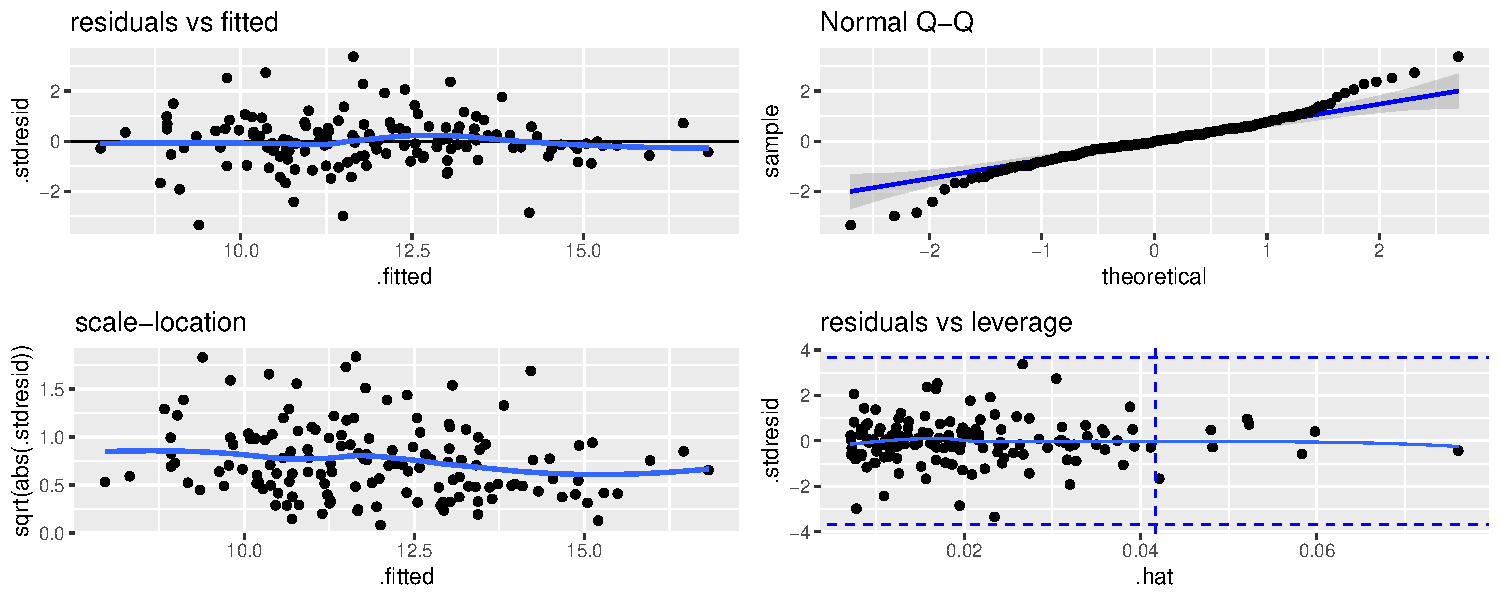
\includegraphics{trabalho_files/figure-pdf/fig-t3-1.pdf}

}

\end{figure}%

\begin{longtable}[t]{l>{\raggedright\arraybackslash}p{17em}r}
\caption{\label{tab:unnamed-chunk-16}Resultados dos Testes de Resíduos}\\
\toprule
Teste & Estatística & p.valor\\
\midrule
Shapiro-Wilk Normality Test & W = 0.96 & 0.0003379\\
Non-constant Variance Score Test & Chisquare = 5.338458 & 0.0208600\\
Durbin-Watson Test for Autocorrelated Errors & D-W Statistic = 2.133801 & 0.4200000\\
\bottomrule
\end{longtable}

Com base na análise da tabela Figura~\ref{fig-t3}, podemos concluir o
seguinte sobre o ajuste do modelo de regressão:

\textbf{Homocedasticidade:} - A variância dos resíduos parece ser
constante em toda a faixa dos valores ajustados, o que é consistente com
a suposição de homocedasticidade na regressão linear.

\textbf{Normalidade:} - Embora o teste de Shapiro-Wilk sugira que os
resíduos não sigam uma distribuição normal, desconsiderando caudas
pesadas tanto nos extremos inferiores quanto nos superiores, podemos
aproximar que os resíduos estão próximos de uma distribuição normal.

\textbf{Independência dos Resíduos:} - Tanto o teste de Durbin-Watson
quanto a inspeção do gráfico de resíduos versus valores ajustados na
tabela Figura~\ref{fig-t3} não fornecem evidências significativas para
rejeitar a hipótese nula de ausência de autocorrelação positiva ou
negativa nos resíduos. Assim, parece que os resíduos são independentes
entre si.

\textbf{Linearidade:} - Não há um padrão claro nos resíduos plotados em
relação aos valores ajustados, indicando linearidade entre as variáveis
independentes e dependentes.

Portanto, concluirmos que o modelo de regressão parece atender às
suposições de homocedasticidade, normalidade aproximada dos resíduos,
independência dos resíduos e linearidade entre as variáveis.

\section{Modelo Gama Log-Linear}\label{modelo-gama-log-linear}

\subsection{Resultados}\label{resultados-1}

Utilizamos o mesmo banco de dados do Modelo de Log-Normal.Por meio da
tabela abaixo é possível verificar como foi o ajuste das variáveis ao
modelo de gama log-linear:

\begin{longtable}[]{@{}lrrrl@{}}

\caption{\label{tbl-gama2}Modelo Gamma Log-linear}

\tabularnewline

\toprule\noalign{}
& Estimacao & ErroPadrao & Pvalor & sig \\
\midrule\noalign{}
\endhead
\bottomrule\noalign{}
\endlastfoot
(Intercept) & 1.6175 & 0.0286 & 0 & \textless0.001*** \\
log(L) & 0.0237 & 0.0032 & 0 & \textless0.001*** \\
log(K) & 0.0601 & 0.0026 & 0 & \textless0.001*** \\

\end{longtable}

O intercepto estimado de 1.61754583 (Tabela~\ref{tbl-gama2}) representa
o logaritmo da produção quando tanto o trabalho (L) quanto o capital (K)
são iguais a 1. Com um p-valor extremamente pequeno, o intercepto é
estatisticamente significativo, indicando que ele desempenha um papel
importante na modelagem da variável dependente 𝑌𝑖, ao nível de 5\% de
significância.

O coeficiente para log(L) é 0.02371, indicando que um aumento de 1\% na
força de trabalho (L) leva a um aumento de aproximadamente 0.024\% na
produção, mantendo o capital constante. O p-valor extremamente pequeno
indica que este coeficiente é altamente significativo, o que valida a
importância da força de trabalho na determinação da produção no modelo.

O coeficiente para log(K) é 0.06012, sugerindo que um aumento de 1\% no
capital (K) resulta em um aumento de aproximadamente 0.060\% na
produção, mantendo a força de trabalho constante. Com um p-valor
extremamente baixo, esse coeficiente é altamente significativo,
demonstrando que o capital tem uma influência importante e
estatisticamente significativa na produção.

O parâmetro de dispersão estimado é 0.00135, o que indica que há uma
baixa variabilidade dos dados em torno da média ajustada pelo modelo.
Isso sugere que o modelo gamma log-linear está capturando bem a
dispersão dos dados, com pouca heterogeneidade residual não explicada
pelo modelo.

\begin{longtable}[t]{l>{\raggedright\arraybackslash}p{17em}}

\caption{\label{tbl-teste}Teste}

\tabularnewline

\toprule
Descrição & Valor\\
\midrule
Soma de alpha e beta & 0.0838\\
Erro padrão & 0.0019\\
Estatística t & -483.1625\\
Valor-p & 7.4303651624535e-229\\
Decisão & Rejeitamos H0\\
\bottomrule

\end{longtable}

Decisão sobre Teste \(𝐻0 : 𝛼 + 𝛽 = 1\) contra \(𝐻1 : 𝛼 + 𝛽 ≠ 1\):
(Tabela~\ref{tbl-teste}) Como o valor-p é extremamente pequeno,
rejeitamos a hipótese nula \(H_0\) indicando que a soma de \(\alpha\) e
\(\beta\) é significativamente diferente de 1. Isso significa que a
hipótese de retornos constantes à escala não é válida para os dados
analisados.

Retornos constantes à escala implicam que, se ambos os insumos (L e K)
aumentarem na mesma proporção, a produção \(Y_i\) também aumentará na
mesma proporção. No entanto, dado que a soma de \(\alpha\) e \(\beta\) é
significativamente diferente de 1, isso sugere que os retornos à escala
não são constantes para este modelo. Dependendo do valor específico da
soma \((\alpha + \beta < 1\) ou \(\alpha + \beta > 1)\), os retornos à
escala podem ser decrescentes ou crescentes, respectivamente.

Assim, a soma de \(\alpha\) e \(\beta\) é 0.08383678, o que está longe
de 1, indicando retornos decrescentes à escala. Isso significa que
aumentar proporcionalmente a força de trabalho e o capital levará a um
aumento menos que proporcional na produção. Em outras palavras, conforme
mais insumos são adicionados, a produtividade marginal desses insumos
diminui, levando a um crescimento menos eficiente da produção.

\subsection{Análise dos Resíduos}\label{anuxe1lise-dos-resuxedduos-1}

\begin{table}

\caption{\label{tbl-gamma1}Gráfico de Análise de resíduos}

\centering{

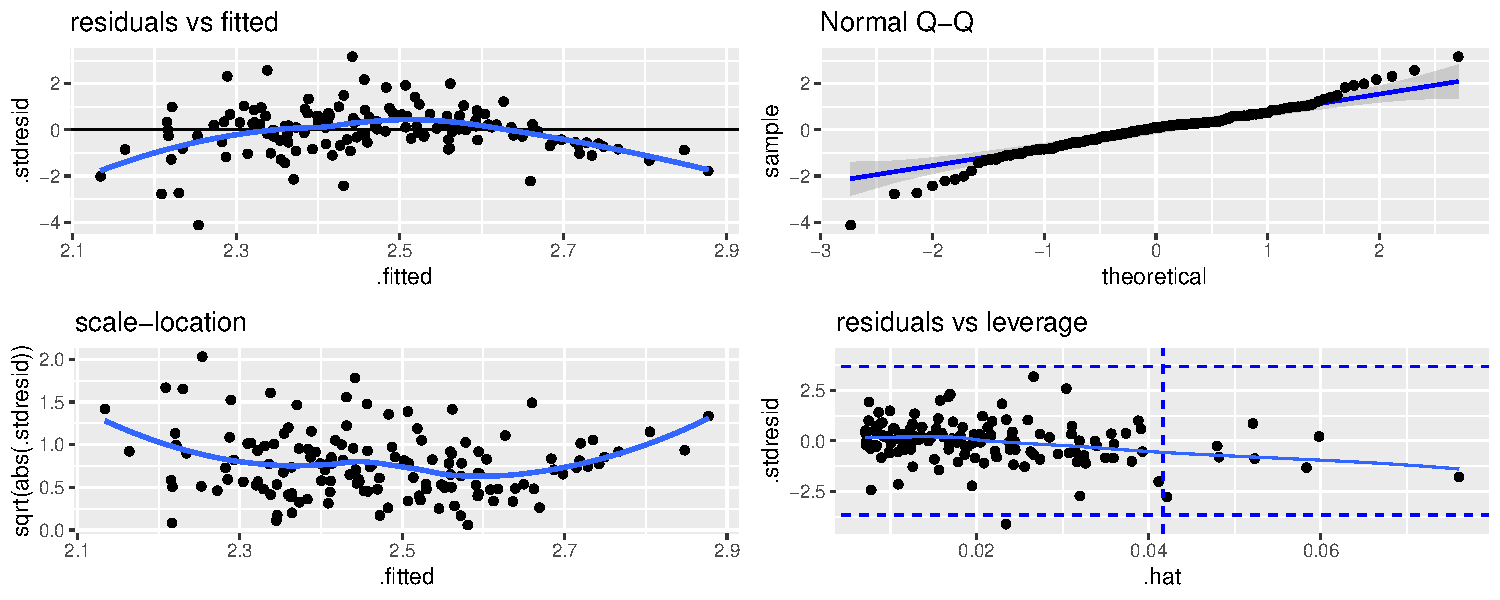
\includegraphics{trabalho_files/figure-pdf/tbl-gamma1-1.pdf}

}

\end{table}%

\begin{longtable}[t]{l>{\raggedleft\arraybackslash}p{17em}rl}
\caption{\label{tab:unnamed-chunk-25}Resultados dos Testes de Breusch-Pagan e Durbin-Watson}\\
\toprule
Teste & Estatística & Valor.p & Decisão\\
\midrule
Breusch-Pagan & 2.6679 & 0.2634 & Não rejeitamos H0\\
Durbin-Watson & 2.1338 & 0.7801 & Não rejeitamos H0\\
\bottomrule
\end{longtable}

Com base na análise dos resíduos, incluindo os testes de Breusch-Pagan e
Durbin-Watson, podemos concluir o seguinte sobre o ajuste do modelo de
regressão:

\textbf{Homocedasticidade:} - A variância dos resíduos parece ser
constante em toda a faixa dos valores ajustados. Com o teste de Teste de
Breusch-Paga, com um valor-p de 0.2634, não rejeitamos a hipótese nula
de homocedasticidade. Isso significa que não há evidências suficientes
para sugerir a presença de heterocedasticidade nos resíduos do modelo
gamma.

\textbf{Normalidade:} - Embora o teste de Shapiro-Wilk sugira que os
resíduos não sigam uma distribuição normal, desconsiderando caudas
pesadas tanto nos extremos inferiores quanto nos superiores, podemos
aproximar que os resíduos estão próximos de uma distribuição normal.

\textbf{Independência dos Resíduos:} - Tanto o teste de Durbin-Watson
quanto a inspeção do gráfico de resíduos versus valores ajustados na
tabela Tabela~\ref{tbl-gamma1} não fornecem evidências significativas
para rejeitar a hipótese nula de ausência de autocorrelação positiva ou
negativa nos resíduos. Assim, parece que os resíduos são independentes
entre si, o que é uma boa indicação de que o modelo está adequadamente
ajustado quanto a essa suposição.

\textbf{Linearidade:} - Há um padrão claro nos resíduos plotados em
relação aos valores ajustados, indicando não linearidade entre as
variáveis independentes e dependentes.

\section{Comparação dos Modelos: Gamma Log-Linear vs.~Modelo
Normal}\label{comparauxe7uxe3o-dos-modelos-gamma-log-linear-vs.-modelo-normal}

\begin{longtable}[t]{l>{\raggedleft\arraybackslash}p{17em}r}
\caption{\label{tab:unnamed-chunk-29}Comparação dos Modelos Gamma Log-Linear e Normal}\\
\toprule
Critério & Modelo.Gamma.Log.Linear & Modelo.Normal\\
\midrule
Log-Likelihood & -83.07791 & -59.39108\\
AIC & 174.15580 & 126.78220\\
BIC & 186.03510 & 138.66140\\
\bottomrule
\end{longtable}

Log-Likelihood (Log-Verossimilhança) - \textbf{Modelo Gamma Log-Linear}:
-83.07791 - \textbf{Modelo Normal}: -59.39108

O valor de log-likelihood mais alto (menos negativo) indica um melhor
ajuste do modelo aos dados. O modelo normal tem um valor de
log-likelihood mais alto, sugerindo que se ajusta melhor aos dados em
comparação com o modelo Gamma log-linear.

Critério de Informação de Akaike (AIC) - \textbf{Modelo Gamma
Log-Linear}: 174.1558 - \textbf{Modelo Normal}: 126.7822

Valores menores de AIC indicam um modelo mais eficiente em termos de
ajuste aos dados com penalização pela complexidade. O modelo normal
apresenta um AIC significativamente menor, indicando que é mais
eficiente e se ajusta melhor aos dados do que o modelo Gamma log-linear.

Critério de Informação de Bayes (BIC) - \textbf{Modelo Gamma
Log-Linear}: 186.0351 - \textbf{Modelo Normal}: 138.6614

O BIC também penaliza a complexidade do modelo e valores menores indicam
um ajuste melhor com menor penalização por complexidade. Novamente, o
modelo normal apresenta um BIC significativamente menor, reforçando que
é mais adequado para os dados em comparação ao modelo Gamma log-linear.

Com base nos critérios de log-likelihood, AIC e BIC, o \textbf{modelo
normal} é a melhor escolha. Ele não só se ajusta melhor aos dados
(conforme indicado pelo log-likelihood), mas também é mais eficiente e
simples em termos de complexidade (conforme indicado pelos valores de
AIC e BIC).

Portanto, o modelo normal é preferível ao modelo Gamma log-linear para a
análise dos seus dados, oferecendo um melhor equilíbrio entre ajuste e
complexidade.

\chapter{Dados Kaggle - análise de clssificação de
crédito}\label{dados-kaggle---anuxe1lise-de-clssificauxe7uxe3o-de-cruxe9dito}

\section{Modelo Logistico}\label{modelo-logistico}

Para este estudo, utilizamos uma base de dados obtida do Kaggle, que
contém informações detalhadas sobre clientes de uma instituição
financeira. O objetivo principal é desenvolver um modelo de machine
learning para classificar o crédito dos clientes em diferentes faixas de
risco, otimizando os processos de decisão e reduzindo esforços manuais.
A base de dados inclui 100.000 observações e 28 variáveis, como idade,
ocupação, renda anual, número de contas bancárias e histórico de
pagamentos.

A análise foca na construção e avaliação de um modelo de
\textbf{regressão logística}, adequado para situações em que a variável
dependente é categórica, como a classificação de crédito (``Poor'' e
``Good''). A \textbf{regressão logística} estima a probabilidade de um
evento binário ocorrer e classifica as observações em categorias. A
equação do modelo logístico é expressa como:

\[log(p / (1 - p)) = β0 + β1 * X_1 + β2 * X_2 + ... + βp * X_p\]

Onde:

\begin{itemize}
\item
  \(p\) é a probabilidade de um cliente ser classificado como ``Good''
  (cliente ser um bom pagador).
\item
  \(1-p\) é a probabilidade de um cliente ser classificado como ``Poor''
  (cliente possui um histórico problemático).
\item
  \(X_1, X_2, ..., X_p\) são as variáveis independentes (como histórico
  de pagamentos, dívida pendente, etc.)
\item
  \(\beta_0, \beta_1, ..., \beta_p\) são os coeficientes que medem o
  impacto de cada variável independente na probabilidade de ser
  classificado como ``Good''.
\end{itemize}

Como parte da análise, será explorado o ajuste do modelo, avaliando os
resíduos para verificar a adequação do modelo.

\begin{longtable}[t]{l>{\raggedright\arraybackslash}p{17em}}
\caption{\label{tab:unnamed-chunk-32}Resumo Descritivo das Variáveis}\\
\toprule
Variável & Estatística\\
\midrule
Credit\_Score & Good: 12192, Poor: 19884\\
Credit\_Mix & Good: 13518, Standard: 8509, Bad: 10049\\
Outstanding\_Debt & Min.: 0.23, 1st Qu.: 702.54, Median: 1360.45, Mean: 1593.26, 3rd Qu.: 2258.30, Max.: 4998.07\\
Payment\_of\_Min\_Amount & No: 14432, Yes: 17644\\
Changed\_Credit\_Limit & Min.: -6.480, 1st Qu.: 4.570, Median: 8.560, Mean: 9.573, 3rd Qu.: 13.130, Max.: 35.820\\
\bottomrule
\end{longtable}

A análise descritiva das variáveis na base de dados dta revela que, dos
32.076 clientes analisados, 12.192 foram classificados como ``Good'' e
19.884 como ``Poor'', indicando que a maioria dos clientes tem uma
classificação de crédito ruim. A variável Credit\_Mix mostra que a
maioria dos clientes tem uma mistura de crédito considerada ``Good'',
seguida por ``Standard'' e ``Bad'', o que pode influenciar a
classificação final de risco. Em relação à dívida pendente, os valores
variam significativamente, com uma mediana de 1.360,45 e uma média de
1.593,26, sugerindo que alguns clientes têm dívidas elevadas, o que pode
aumentar o risco de crédito. Quanto ao pagamento do valor mínimo, 17.644
clientes o fizeram, enquanto 14.432 não, indicando que pagar apenas o
valor mínimo pode ser um indicador de problemas financeiros. A variável
Changed\_Credit\_Limit mostra variações entre -6,48 e 35,82, com uma
mediana de 8,56, sugerindo mudanças no comportamento de crédito ao longo
do tempo. Essas observações iniciais são fundamentais para a construção
do modelo de regressão logística e devem orientar a escolha de variáveis
e a interpretação dos resultados.

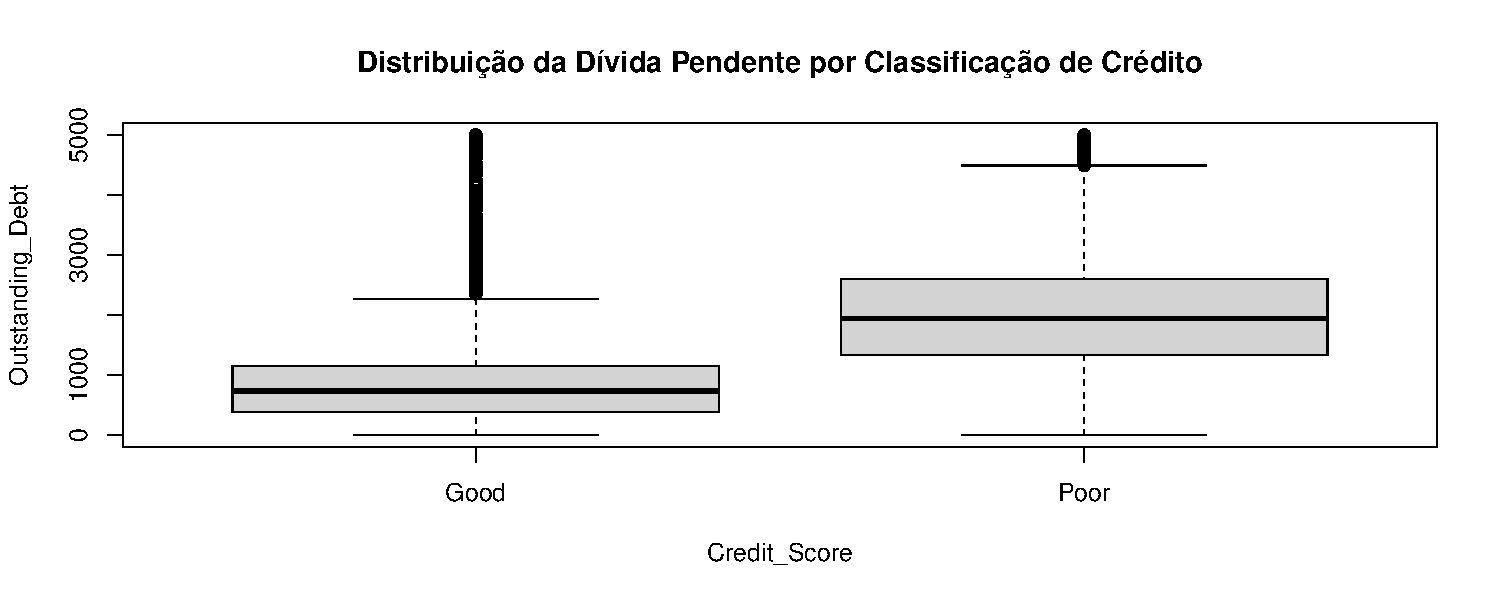
\includegraphics{trabalho_files/figure-pdf/unnamed-chunk-33-1.pdf}

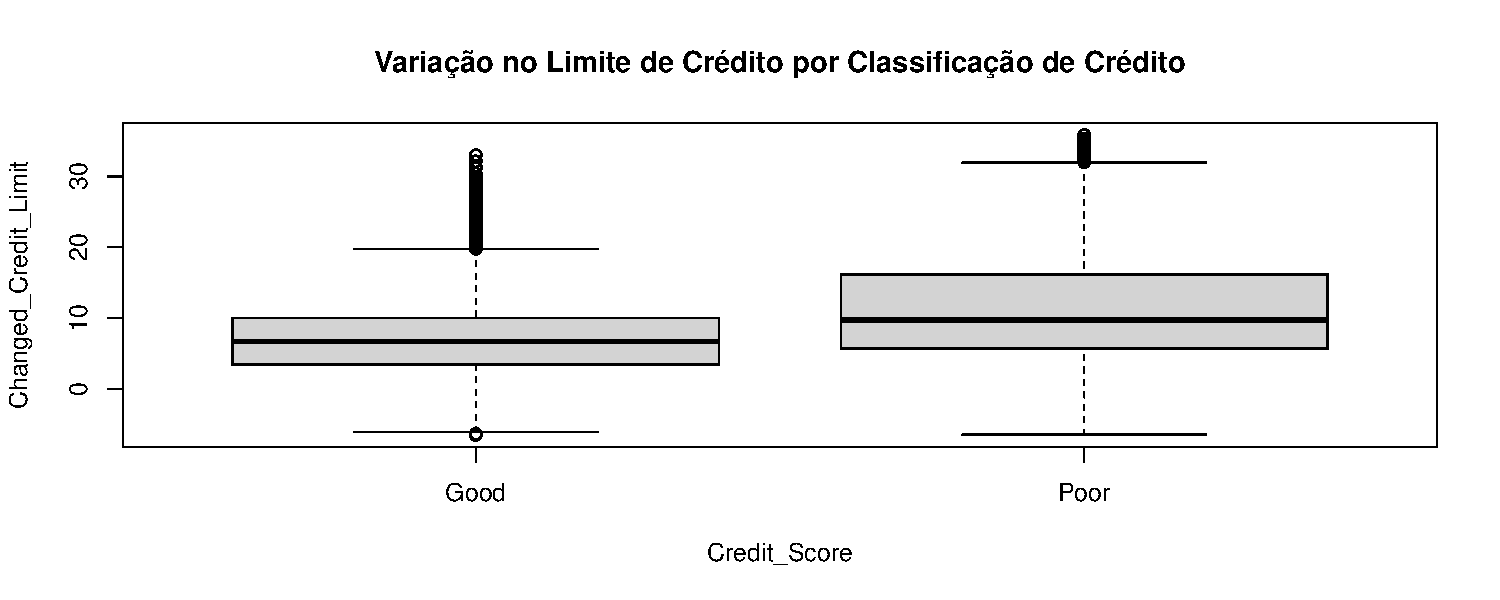
\includegraphics{trabalho_files/figure-pdf/unnamed-chunk-33-2.pdf}

\begin{longtable}[t]{lrrll}
\caption{\label{tab:unnamed-chunk-34}Resultados dos Testes Qui-Quadrado}\\
\toprule
Teste & Estatística & Graus.de.Liberdade & Valor.p & Decisão\\
\midrule
Credit\_Mix vs Credit\_Score & 14606 & 2 & < 2.2e-16 & Rejeitamos H0\\
Payment\_of\_Min\_Amount vs Credit\_Score & 14578 & 1 & < 2.2e-16 & Rejeitamos H0\\
\bottomrule
\end{longtable}

A análise associativa preliminar entre as variáveis do estudo revela
insights importantes sobre os padrões de crédito dos clientes. Através
dos boxplots, observa-se que a dívida pendente (Outstanding\_Debt) tende
a ser maior entre os clientes com uma classificação de crédito ``Poor''
em comparação com aqueles classificados como ``Good''. Isso sugere que
clientes com maiores dívidas são mais propensos a terem uma
classificação de crédito inferior. Além disso, as mudanças no limite de
crédito (Changed\_Credit\_Limit) também variam significativamente entre
as classificações de crédito, com clientes de crédito ``Poor'' exibindo
maior variação, o que pode indicar instabilidade financeira.

As análises de qui-quadrado entre as variáveis categóricas reforçam
essas observações. O teste de associação entre a mistura de crédito
(Credit\_Mix) e a classificação de crédito (Credit\_Score) resultou em
um valor de X² de 14.606 com um p-valor extremamente significativo
(\textless{} 2,2e-16), indicando uma forte associação entre essas
variáveis. Isso sugere que a composição do crédito do cliente tem uma
influência considerável sobre sua classificação de crédito. De forma
similar, o teste de qui-quadrado entre o pagamento do valor mínimo
(Payment\_of\_Min\_Amount) e a classificação de crédito também mostrou
uma associação significativa (X² = 14.578, p \textless{} 2,2e-16),
sugerindo que clientes que não pagam o valor mínimo regularmente têm
maior probabilidade de serem classificados como ``Poor''. Esses
resultados preliminares fornecem evidências robustas de que variáveis
financeiras e comportamentais desempenham um papel crucial na
determinação do risco de crédito, justificando sua inclusão no modelo de
regressão logística subsequente.

\subsection{Modelo logístico
ajustado}\label{modelo-loguxedstico-ajustado}

O modelo de regressão logística ajustado para classificar o crédito dos
clientes foi desenvolvido utilizando A função de link utilizada foi a
logit, adequada para a análise de variáveis binárias como o
Credit\_Score.

Além disso, para a construção do modelo foram utilizadas as seguintes
variáveis:

\begin{longtable}[t]{lrrl}
\caption{\label{tab:unnamed-chunk-35}Resultados do Modelo de Regressão Logística}\\
\toprule
Variável & Estimacao & ErroPadrao & Pvalor\\
\midrule
(Intercept) & -1.4850888 & 0.0361200 & < 0.05\\
Credit\_MixStandard & 1.0098831 & 0.0701266 & < 0.05\\
Credit\_MixBad & 2.3447565 & 0.1036433 & < 0.05\\
Outstanding\_Debt & 0.0006567 & 0.0000294 & < 0.05\\
Payment\_of\_Min\_AmountYes & 1.4233394 & 0.0804651 & < 0.05\\
\addlinespace
Changed\_Credit\_Limit & -0.0238181 & 0.0036734 & < 0.05\\
\bottomrule
\end{longtable}

Os coeficientes do modelo são significativos, com valores de p
inferiores a 0,05 para todas as variáveis, indicando que elas têm uma
contribuição estatisticamente significativa na previsão da classificação
de crédito.

Aqui, o intercepto é −1.485, enquanto os coeficientes para as variáveis
Credit\_MixStandard e Credit\_MixBad são positivos e relativamente
altos, o que sugere um efeito significativo na probabilidade de um
cliente ser classificado como ``Good''. Outstanding\_Debt e
Payment\_of\_Min\_AmountYes também apresentam coeficientes positivos,
refletindo seu impacto positivo na probabilidade de uma boa
classificação de crédito. O coeficiente de Changed\_Credit\_Limit é
negativo, indicando que um aumento no limite de crédito alterado está
associado a uma menor probabilidade de classificação positiva.

O modelo apresenta um desvio nulo de 42604 e um desvio residual de
24833. A redução no desvio residual em relação ao desvio nulo indica que
o modelo com as variáveis independentes tem um ajuste significativamente
melhor do que o modelo nulo. Em outras palavras, o modelo ajustado reduz
a discrepância entre os valores previstos e os observados de forma
significativa.

Quanto ao AIC, vale salientar que O AIC é uma métrica que ajuda a
avaliar a qualidade do ajuste do modelo, levando em consideração tanto a
complexidade quanto a adequação ao conjunto de dados. A principal função
do AIC é penalizar modelos mais complexos, que possuem um maior número
de parâmetros, para evitar o ajuste excessivo aos dados (overfitting).No
caso, o AIC obtido foi de 24845. Para determinar se este valor indica um
bom ajuste do modelo, é necessário compará-lo com o AIC de outros
modelos que você pode ter testado.

Para o modelo ajustado foi calculado também a razão de chances:

\begin{longtable}[]{@{}lr@{}}
\caption{Razões de Chances (Odds Ratios) do Modelo de Regressão
Logística}\tabularnewline
\toprule\noalign{}
& Odds\_Ratio \\
\midrule\noalign{}
\endfirsthead
\toprule\noalign{}
& Odds\_Ratio \\
\midrule\noalign{}
\endhead
\bottomrule\noalign{}
\endlastfoot
(Intercept) & 0.226 \\
Credit\_MixStandard & 2.745 \\
Credit\_MixBad & 10.431 \\
Outstanding\_Debt & 1.001 \\
Payment\_of\_Min\_AmountYes & 4.151 \\
Changed\_Credit\_Limit & 0.976 \\
\end{longtable}

As razões de chances (odds ratios) para o modelo de regressão logística
ajustado fornecem uma visão sobre como cada variável preditora afeta a
probabilidade de uma boa classificação de crédito. As variáveis
``Credit\_MixStandard'' e ``Credit\_MixBad'' têm odds ratios de
aproximadamente 2.75 e 10.43, respectivamente, indicando que os
indivíduos com essas classificações de crédito têm odds
significativamente maiores de obter uma boa classificação em comparação
com a categoria de referência. O valor da dívida pendente
(``Outstanding\_Debt'') tem um odds ratio próximo de 1, sugerindo que
sua influência nas odds é mínima. Por outro lado, pagar o valor mínimo
requerido (``Payment\_of\_Min\_AmountYes'') aumenta as odds de uma boa
classificação de crédito em cerca de 4.15 vezes. O limite de crédito
alterado (``Changed\_Credit\_Limit'') tem um odds ratio de 0.98,
indicando uma leve diminuição nas odds de uma boa classificação com cada
unidade adicional de alteração no limite de crédito. Esses resultados
ajudam a entender a importância relativa de cada variável na previsão da
classificação de crédito.

Tentamos ajustar o modelo logistico, re-escalando Outstanding Debt:

\begin{longtable}[t]{lrrl}
\caption{\label{tab:unnamed-chunk-37}Resultados do Modelo de Regressão Logística}\\
\toprule
Variável & Estimacao & ErroPadrao & Pvalor\\
\midrule
(Intercept) & -1.4850888 & 0.0361200 & < 0.05\\
Credit\_MixStandard & 1.0098831 & 0.0701266 & < 0.05\\
Credit\_MixBad & 2.3447565 & 0.1036433 & < 0.05\\
Outstanding\_Debt\_scaled & 0.0656720 & 0.0029353 & < 0.05\\
Payment\_of\_Min\_AmountYes & 1.4233394 & 0.0804651 & < 0.05\\
\addlinespace
Changed\_Credit\_Limit & -0.0238181 & 0.0036734 & < 0.05\\
\bottomrule
\end{longtable}

Visando verificar se é possível melhorar o modelo logístico ajustado, a
variável Outstanding\_Debt foi recalibrada. No modelo anterior, o
coeficiente para Outstanding\_Debt era muito pequeno (6.567e-04),
enquanto no modelo ajustado com a variável escalada
(Outstanding\_Debt\_scaled), a estimativa do coeficiente foi
significativamente maior (0.065672), indicando um efeito mais expressivo
da variável escalada. No entanto, apesar de a escalagem ter melhorado a
interpretação dos coeficientes, os desvios nulo e residual, assim como o
AIC, permaneceram inalterados (o AIC é 24845 para ambos os modelos).
Isso sugere que, embora a escalagem tenha proporcionado coeficientes
mais interpretáveis, ela não resultou em uma melhoria no ajuste global
do modelo.

\subsection{Análise dos Resíduos}\label{anuxe1lise-dos-resuxedduos-2}

A análise dos resíduos é crucial para avaliar se o modelo logístico está
bem ajustado. Resíduos bem comportados, ou seja, sem padrões claros e
distribuídos de forma aleatória, indicam que o modelo é adequado. Se
houver padrões nos resíduos, isso pode sugerir que o modelo não está
capturando toda a variabilidade dos dados, podendo haver variáveis
importantes faltantes ou problemas de especificação do modelo

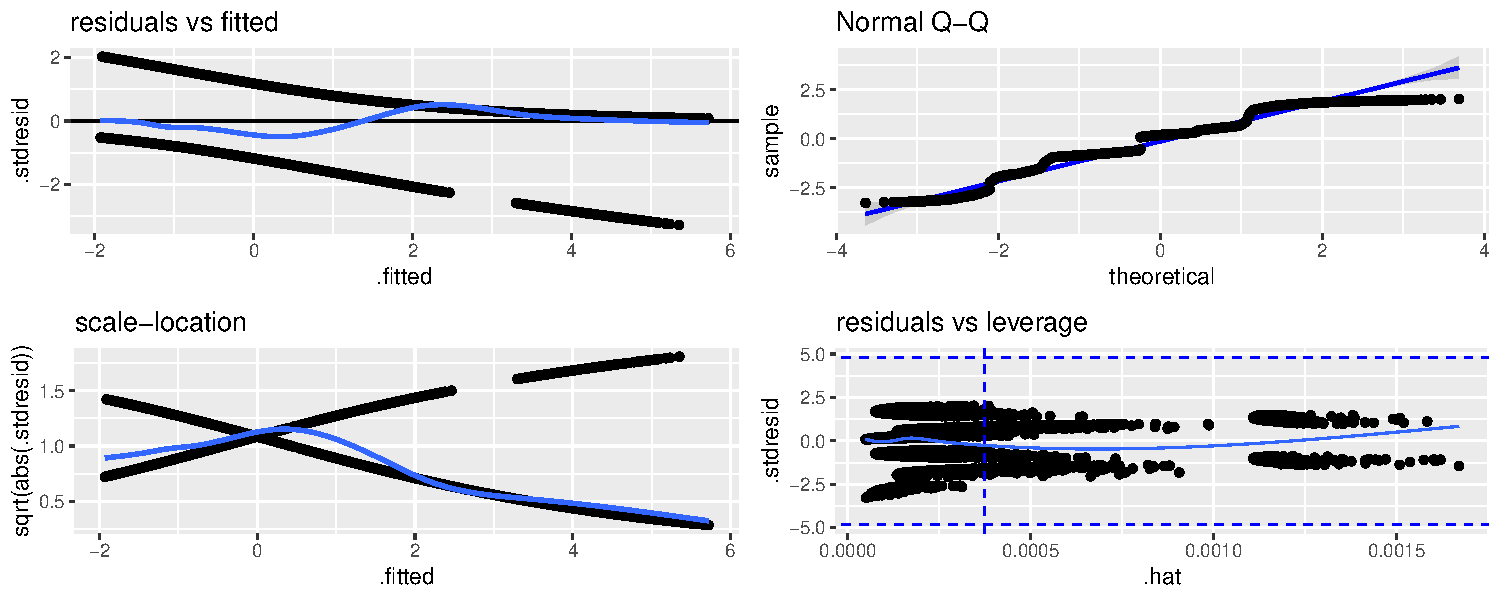
\includegraphics{trabalho_files/figure-pdf/unnamed-chunk-38-1.pdf}

\begin{longtable}[t]{llll}
\caption{\label{tab:unnamed-chunk-40}Resultados dos Testes Breusch-Pagan e Durbin-Watson}\\
\toprule
Teste & Estatistica & Graus\_de\_Liberdade & P\_valor\\
\midrule
Breusch-Pagan & BP = 3931.9 & df = 5 & p-value < 2.2e-16\\
Durbin-Watson & DW = 0.65232 & NA & p-value < 2.2e-16\\
\bottomrule
\end{longtable}

Com base nos resultados obtidos via Teste de Breusch-Pagan e Teste de
Durbin-Watson, podemos concluir o seguinte sobre o ajuste do modelo de
regressão logística:

\textbf{Homocedasticidade:} - O Teste de Breusch-Pagan resultou em um
valor de BP = 3931.9 com um valor-p \textless{} 2.2e-16. Esse valor-p
extremamente baixo indica que rejeitamos a hipótese nula de
homocedasticidade. Em outras palavras, há evidências significativas de
heterocedasticidade nos resíduos do modelo. Isso sugere que a variância
dos resíduos não é constante ao longo dos valores preditores, o que pode
indicar que o modelo não está capturando completamente a variabilidade
dos dados.

\textbf{Independência dos Resíduos:} - O Teste de Durbin-Watson forneceu
um valor de DW = 0.65232 com um valor-p \textless{} 2.2e-16, indicando
uma forte presença de autocorrelação positiva nos resíduos. Isso sugere
que os resíduos não são independentes entre si, o que pode indicar que o
modelo não está capturando todos os padrões nos dados ou que há uma
estrutura de dependência não modelada.

A inspeção do gráfico de resíduos versus valores ajustados também pode
revelar padrões adicionais que confirmem a presença de autocorrelação.

\textbf{Linearidade:} - Há um padrão claro nos resíduos plotados em
relação aos valores ajustados, indicando não linearidade entre as
variáveis independentes e dependentes.

Desse modo, os resultados sugerem que o modelo enfrenta problemas de
heterocedasticidade e autocorrelação positiva dos resíduos, o que pode
impactar a precisão e a validade do modelo.

\subsection{Análise do VIF (Variance Inflation
Factor)}\label{anuxe1lise-do-vif-variance-inflation-factor}

O VIF (Fator de Inflação da Variância) é uma medida importante para
identificar a presença de multicolinearidade entre os preditores em um
modelo de regressão. Valores elevados de VIF sugerem que um preditor
está altamente correlacionado com outros preditores no modelo, o que
pode inflacionar os erros padrão das estimativas dos coeficientes e
dificultar a identificação da real significância das variáveis.

\begin{longtable}[t]{lrrr}
\caption{\label{tab:unnamed-chunk-41}VIF dos Preditores}\\
\toprule
Preditor & GVIF & Df & Ajuste.do.GVIF\\
\midrule
Credit\_Mix & 5.405144 & 2 & 1.524761\\
Outstanding\_Debt & 1.626080 & 1 & 1.275178\\
Payment\_of\_Min\_Amount & 5.496045 & 1 & 2.344365\\
Changed\_Credit\_Limit & 1.558789 & 1 & 1.248515\\
\bottomrule
\end{longtable}

\begin{longtable}[t]{lr}
\caption{\label{tab:unnamed-chunk-42}Erros Padrão dos Coeficientes}\\
\toprule
Coeficiente & Erro\_Padrão\\
\midrule
Intercept & 0.0361200\\
Credit\_MixStandard & 0.0701266\\
Credit\_MixBad & 0.1036433\\
Outstanding\_Debt & 0.0000294\\
Payment\_of\_Min\_AmountYes & 0.0804651\\
\addlinespace
Changed\_Credit\_Limit & 0.0036734\\
\bottomrule
\end{longtable}

No modelo analisado, observamos que as variáveis Credit\_Mix e
Payment\_of\_Min\_Amount têm VIFs relativamente altos, com valores de
5.41 e 5.50, respectivamente. Esses valores indicam uma alta
colinearidade com outras variáveis do modelo. Isso é corroborado pelos
erros padrão dos coeficientes: Credit\_MixStandard e Credit\_MixBad
apresentam erros padrão elevados, especialmente Credit\_MixBad com um
erro padrão de 0.1036, o que sugere que as estimativas dos coeficientes
para estas variáveis são menos precisas e podem ser afetadas pela
multicolinearidade.

Em contraste, Outstanding\_Debt e Changed\_Credit\_Limit têm VIFs
baixos, de 1.63 e 1.56, respectivamente. Isso sugere que estas variáveis
têm baixa colinearidade com outras variáveis do modelo. O erro padrão
para Outstanding\_Debt é extremamente pequeno (aproximadamente 0.0000),
indicando uma estimativa muito precisa para o coeficiente desta
variável. Da mesma forma, Changed\_Credit\_Limit tem um erro padrão
muito pequeno (0.0037), o que também sugere uma estimativa precisa para
o coeficiente desta variável.

Por outro lado, o erro padrão para Payment\_of\_Min\_AmountYes é
relativamente grande (0.0805), o que pode refletir a alta
multicolinearidade observada pelo VIF elevado para
Payment\_of\_Min\_Amount. Isso indica que a estimativa do coeficiente
para esta variável pode ser menos confiável.

Em resumo, a alta multicolinearidade identificada para Credit\_Mix e
Payment\_of\_Min\_Amount está associada a erros padrão mais altos para
essas variáveis, o que sugere que as estimativas dos coeficientes podem
ser imprecisas. Em contraste, variáveis com VIFs baixos como
Outstanding\_Debt e Changed\_Credit\_Limit apresentam erros padrão
menores e estimativas mais confiáveis. Considerar a remoção ou ajuste
das variáveis com alta colinearidade pode melhorar a precisão e robustez
do modelo.



\end{document}
